\chapter{Design}

\section{Overall System Design}

\subsection{Short description of the main parts of the system}

\begin{itemize}
	\item \textbf{GCSE Trigonometry and Pythagoras Education System:}
	\begin{itemize}
		\item General User Interface
		\item Getting Username and Password
		\item Navigating User's Personal Account User Interface
		\item Setting Homework From Administrator
		\item Running Individual Lessons
		\item Running Individual Homeworks
		\item Accepting User Inputs
		\item Outputting Error Exception Messages
		\item Recording Homework Results On Database
	\end{itemize}
\end{itemize}

\begin{itemize}
	\item General User Interface
	\begin{itemize}
		\item This is the general layout of the interface across the system; the same layout pattern, same colour scheme, same positioning design.
		\item This will provide the user with the ability to navigate the parts of the system that they have access to, and enable them to select tasks, submit homeworks, and access the database to view their personal and homework records.
	\end{itemize}
\end{itemize}

\begin{itemize}
	\item Getting Username and Password
	\begin{itemize}
		\item This will come in the very first window every time the user or administrator wants to access the program; it will ask them to log in so that they can view their own personal account, with all of their homework progress and personal records.
		\item It will mainly consist of two text boxes in the centre of the screen, one prompting a username and the other a password underneath. 
		\item If invalid information is input it will display an error message asking the user to retry. There will be no limit to the number of attempts a user can have; it won't lock them out of their computer if they keep getting it wrong.
	\end{itemize}
\end{itemize}

\begin{itemize}
	\item Navigating User's Personal Account User Interface
	\begin{itemize}
		\item This is essentially the functionality between each window. The user will have a range of buttons to press which will then open the relevant window, and then will have the option to return, making each part of the system accessible.
	\end{itemize}
\end{itemize}

\begin{itemize}
	\item Setting Homework From Administrator
	\begin{itemize}
		\item The function which makes the user aware of which homework has been set; the administrator will set it, the system will acknowledge it, and then notify the required users to do it.
		\item The reverse will work similarly; the user will complete the homework and the administrator will be notified. They will also be notified if the user hasn't completed it before the due date.
	\end{itemize}
\end{itemize}

\begin{itemize}
	\item Running Individual Lessons
	\begin{itemize}
		\item The module that runs for each lesson. Each lesson will have its own set of windows, containing the inputs, outputs and graphics to accurately represent what is being taught e.g Pythagoras Theorem.
		\item These will only be opened, navigated and closed as nothing from these is recorded in the database; they are effectively read only.
	\end{itemize}
\end{itemize}

\begin{itemize}
	\item Running Individual Homeworks
	\begin{itemize}
		\item The module that runs for each homework, saved so that each different homework task is always the same, in order to avoid confusion. 
		\item When the homework is run, inputs are accepted, outputs are given, and at the end the appropriate information is recorded in the database.
	\end{itemize}
\end{itemize}

\begin{itemize}
	\item Accepting User Inputs
	\begin{itemize}
		\item Each input type in the system, be it the general user interface, a lesson or a homework, will be accepted.
		\item Once accepted, it will be validated, and if invalid, the appropriate error mesage will be displayed.
		\item Different types of inputs are:
		\begin{itemize}
			\item Text Boxes
			\item Drag and Drop Images
			\item Image Modification
			\item Buttons 
		\end{itemize} 
		\item If valid, the system will either allow them access to their account, or add a mark to their homework task score.
	\end{itemize}
\end{itemize}

\begin{itemize}
	\item Outputting Error Exception Messages
	\begin{itemize}
		\item If a user's input is invalid, the appropriate error message will be displayed.
		\item Each error message will appear for 5 seconds and then disappear automatically.
		\item These are the variations of error messages and their causes:
		\begin{itemize}
			\item Invalid Username
			\item Invalid Password
			\item Invalid Data Type
			\item Wrong Answer 1{$^s$}{$^t$}
			\item Wrong Answer 2{$^n$}{$^d$}
			\item Unauthorised Access
		\end{itemize}
	\end{itemize}
\end{itemize}

\begin{itemize}
	\item Recording Homework Results On Database
	\begin{itemize}
		\item Every time a user completes a homework, the results will be recorded in the database, including the \textbf{OverallPercentScore}, \textbf{IndividualPercentScore(s)}, and \textbf{Rating}. 
		\item The user will be able to view their results in their personal database section, and the administrator will be able to view these results in the entire class database for that task.
	\end{itemize}
\end{itemize}

\subsection{System flowcharts showing an overview of the complete system}

\textbf{This flowchart represents the system accessible for a student/user: }

\begin{figure}[H]
    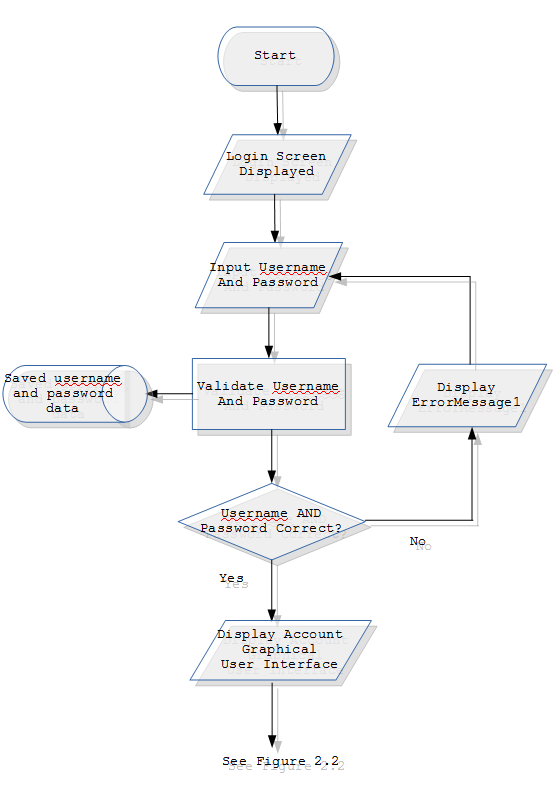
\includegraphics[width=\textwidth]{C:/Users/Jordan/git/COMP4Coursework2/user_flow_1}
    \label{fig:print_function_result}\caption{}
\end{figure}

\begin{figure}[H]
    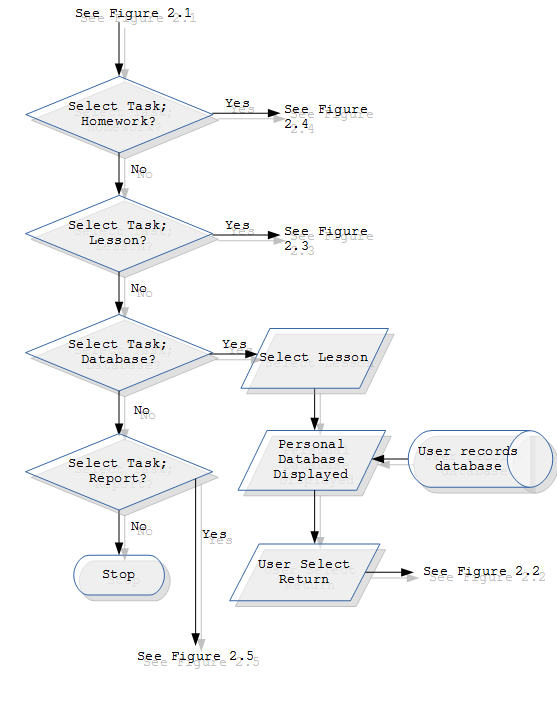
\includegraphics[width=\textwidth]{C:/Users/Jordan/git/COMP4Coursework2/user_flow_2}
    \label{fig:print_function_result}\caption{}
\end{figure}

\begin{figure}[H]
    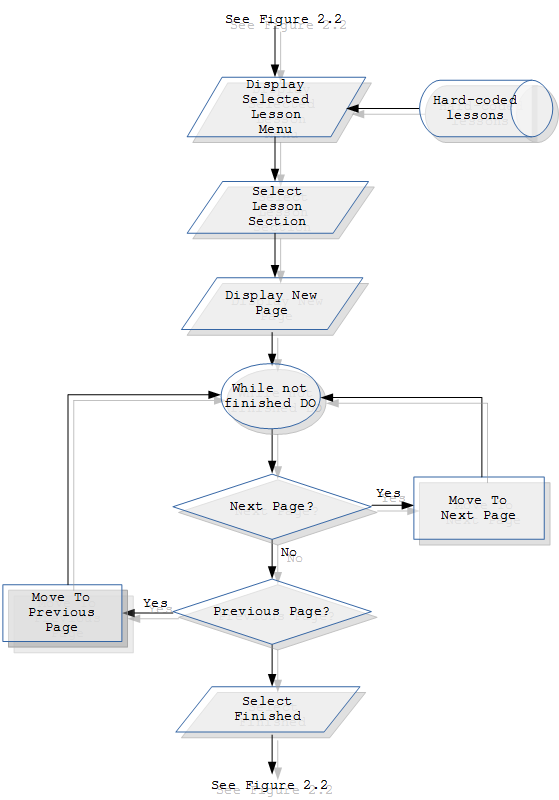
\includegraphics[width=\textwidth]{C:/Users/Jordan/git/COMP4Coursework2/user_flow_3}
    \label{fig:print_function_result}\caption{}
\end{figure}

\begin{figure}[H]
    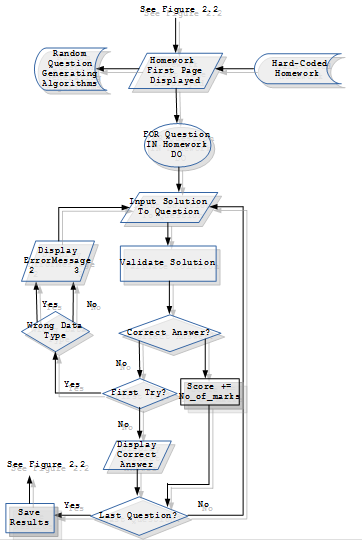
\includegraphics[width=\textwidth]{C:/Users/Jordan/git/COMP4Coursework2/user_flow_4}
    \label{fig:print_function_result}\caption{}
\end{figure}

\textbf{This flowchart represents the system accessible for a teacher/administrator: }

\begin{figure}[H]
    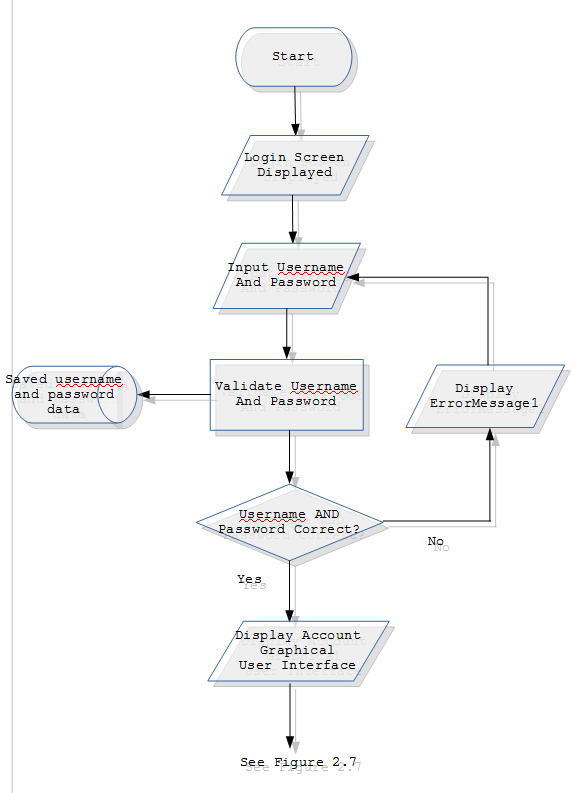
\includegraphics[width=\textwidth]{C:/Users/Jordan/git/COMP4Coursework2/admin_flow_1}
    \label{fig:print_function_result}\caption{}
\end{figure}

\begin{figure}[H]
    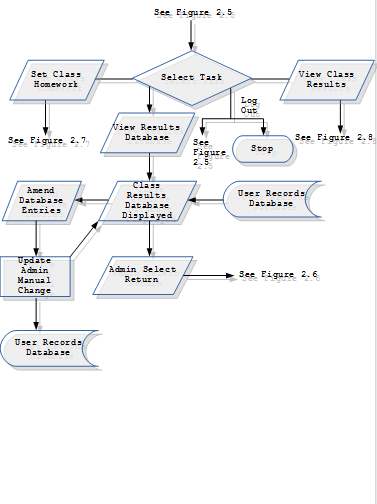
\includegraphics[width=\textwidth]{C:/Users/Jordan/git/COMP4Coursework2/admin_flow_2}
    \label{fig:print_function_result}\caption{}
\end{figure}

\begin{figure}[H]
    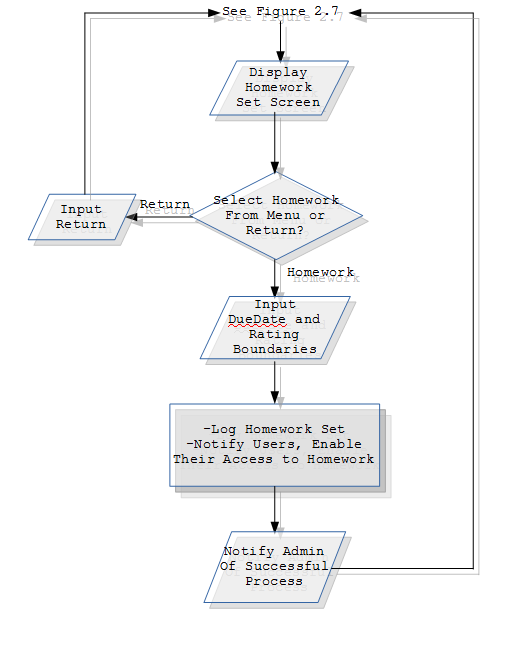
\includegraphics[width=\textwidth]{C:/Users/Jordan/git/COMP4Coursework2/admin_flow_3}
    \label{fig:print_function_result}\caption{}
\end{figure}

\begin{figure}[H]
    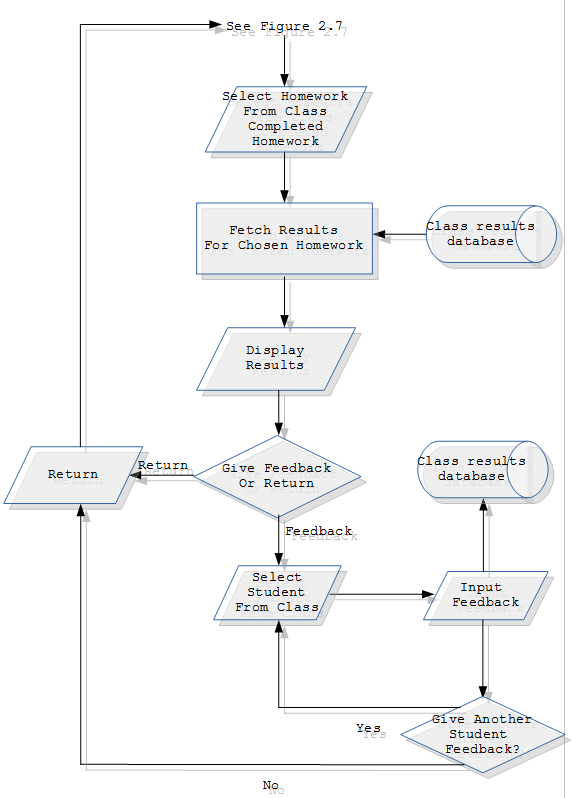
\includegraphics[width=\textwidth]{C:/Users/Jordan/git/COMP4Coursework2/admin_flow_4}
    \label{fig:print_function_result}\caption{}
\end{figure}

\section{User Interface Designs}



\section{Hardware Specification}

\section{Program Structure}

\subsection{Top-down design structure charts}

\subsection{Algorithms in pseudo-code for each data transformation process}

\subsection{Object Diagrams}

\subsection{Class Definitions}

\section{Prototyping}

\section{Definition of Data Requirements}

\subsection{Identification of all data input items}

\subsection{Identification of all data output items}

\subsection{Explanation of how data output items are generated}

\subsection{Data Dictionary}

\subsection{Identification of appropriate storage media}

\section{Database Design}

\subsection{Normalisation}

\subsubsection{ER Diagrams}

\subsubsection{Entity Descriptions}

\subsubsection{1NF to 3NF}

\subsection{SQL Queries}

\section{Security and Integrity of the System and Data}

\subsection{Security and Integrity of Data}

\subsection{System Security}

\section{Validation}

\section{Testing}

\begin{landscape}
\subsection{Outline Plan}

\begin{center}
    \begin{tabular}{|p{2cm}|p{5cm}|p{5cm}|p{4cm}|}
        \hline
        \textbf{Test Series} & \textbf{Purpose of Test Series} & \textbf{Testing Strategy} & \textbf{Strategy Rationale}\\ \hline
        Example & Example & Example & Example \\ \hline
    \end{tabular}
\end{center}

\subsection{Detailed Plan}

\begin{center}
    \begin{longtable}{|p{1.5cm}|p{2.5cm}|p{2.5cm}|p{2cm}|p{2cm}|p{2cm}|p{2cm}|p{2cm}|}
        \hline
        \textbf{Test Series} & \textbf{Purpose of Test} & \textbf{Test Description} & \textbf{Test Data} & \textbf{Test Data Type (Normal/ Erroneous/ Boundary)} & \textbf{Expected Result} & \textbf{Actual Result} & \textbf{Evidence}\\ \hline
        Example & Example & Example & Example & Example & Example & Example & Example \\ \hline
    \end{longtable}
\end{center}
\end{landscape}